\documentclass[twoside,10pt]{article}
\usepackage{shlists}
\usepackage[applemac]{inputenc}
\usepackage[spanish]{babel}
\usepackage[T1]{fontenc}


\usepackage{multicol}
\usepackage{picinpar}

\usepackage{url}
\newcommand{\surl}[1]{{\small\url{#1}}}

\newcounter{vol}
\newcounter{num}
\newcounter{anyo}
\setcounter{vol}{9}
\setcounter{num}{2}
\setcounter{anyo}{2016}
\newcommand{\mes}{Mayo}
\usepackage{revisionNLcol}


\title{\ \\ Docencia 2.0\\ \large Juan Juli\'{a}n Merelo, Fernando Tricas}
\author{\LARGE Lenguajes de programaci\'on: ?`uno, ninguno o todos?}

\date{}

\AutTit{Docencia 2.0}

\begin{document}
\addtocounter{page}{2}

\maketitle

\vspace*{-5ex}

\begin{multicols}{2}

Si hay un tema transversal en la inform\'atica son los lenguajes de
programaci\'on. Desde los niveles m\'as bajos de la arquitectura a los m\'as
altos, la forma universal en la que el ser humano se comunica con un
ordenador son los programas, escritos en alguno de los lenguajes de
programaci\'on disponibles. Los lenguajes suelen tener una serie de
caracter\'{\i}sticas comunes: una sintaxis r\'{\i}gida, implementaciones con
licencia libre y una evoluci\'on continua.

En esta \'ultima caracter\'{\i}stica est\'a uno de los problemas. El lenguaje
que ense\~{n}aste en primero puede no parecerse en nada al que usar\'as en
el trabajo de fin de grado. Pero si consideramos que la evoluci\'on
individual est\'a acompa\~{n}ada de una evoluci\'on colectiva de los tipos de
lenguajes que se usan y que, por tanto, se necesitan no ya para
conseguir un puesto de trabajo, sino siquiera para poder trabajar en
un entorno de computaci\'on determinado, la elecci\'on de un lenguaje de
programaci\'on para una asignatura o para una carrera entera se convierte en
una tarea ardua o imposible.

Porque, seamos pr\'acticos, elegir un solo lenguaje para regirlos a
todos es imposible en nuestro pa\'{\i}s. Ni en ninguno, para el caso.
Nuestra idiosincrasia impedir\'{\i}a que m\'as de dos personas se pusieran de
acuerdo en qu\'e lenguaje usar desde primero a cuarto, y en el caso
improbable de que un {\em ukase} de la superioridad impusiera uno, esa
misma idiosincrasia har\'{\i}a que el profesor de pr\'acticas de tercero usara
eventualmente el que le viniera en gana. 
Seguramente esto es hasta sano y saludable porque, ?`qui\'en nos asegurar\'{\i}a
que en el `mundo real' la sociedad y la industria habr\'{\i}a elegido este
supuesto lenguaje ganador y tan perfecto para habernos puesto de acuerdo a
nosotros? Habr\'a que agradecerle al profesor de pr\'acticas de tercero el que
el alumno  haya tenido exposici\'on a diversos lenguajes y
entornos de trabajo. Por esa misma raz\'on descartamos esa opci\'on
del lenguaje \'unico y puro para dominarlos a todos.

Tambi\'en podr\'{\i}amos pensar, siguiendo las metodolog\'{\i}as modernas, la idea de
adaptaci\'on al estudiante: cada cu\'al que elija su lenguaje favorito y que lo
utilice
para desarrollar sus proyectos. Seguramente nos encontrar\'{\i}amos con algunas
dificultades: lenguajes poco adecuados para las tareas que est\'an
relacionadas con la tem\'atica de la asignatura, excesivo `monocultivo',
dado que es f\'acil ponerse de acuerdo con uno mismo y terminar haciendo todo
con una sola tecnolog\'{\i}a (perdiendo en el camino la oportunidad de
explorar otras), y la
no despreciable complejidad de prestar asistencia en caso de alguna cosa no
vaya bien. 

Desde nuestra experiencia esta puede ser una buena aproximaci\'on cuando
vamos avanzando en la carrera: Sugerir, por ejemplo, un lenguaje que
nosotros creamos adecuado pero facilitar que se elijan alternativas.
Eventualmente, el profesor no tiene que evaluar al
alumno por la letra de lo que haya hecho, es decir, la literalidad de
haber escrito alg\'un algoritmo o usado una estructura de datos en un
lenguaje que el profesor conoce, sino por el hecho de que haya sido
capaz de entender esos conceptos y usarlos en la pr\'actica. No
resultar\'{\i}a dif\'{\i}cil, para cualquier profesor, evaluar la consecuci\'on de
los objetivos por parte del alumno en casi cualquier lenguaje de
programaci\'on. Salvo, quiz\'a, Haskell.

Vamos avanzando.


%--------------------------
\noindent\rule{86mm}{1pt}
\vspace{1ex} {\small{\begin{window}[0,r,
\includegraphics[width = 27mm]{JJM.jpg},] 
\noindent\emph{JJ Merelo} es catedr\'{a}tico de Universidad
en el \'area de Arquitectura y Tecnolog\'{\i}a de Computadores, y
actualmente director de la Oficina de Software Libre de la UGR.
\'{U}ltimamente le ha dado por el \textsl{flipped
learning}, de lo que se informar\'{a} debidamente en esta columna.
\end{window}}} 
\medskip

{\small{\begin{window}[0,r,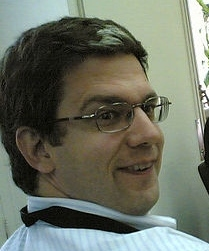
\includegraphics[width = 27 mm]{FTricas1.jpg},]
		\noindent \emph{Fernando Tricas Garc\'{\i}a} es profesor
		titular de Lenguajes y Sistemas Inform\'{a}ticos del Departamento
		de Inform\'{a}tica e Ingenier\'{\i}a de Sistemas de la Universidad de
		Zaragoza.  Empez\'{o} a estudiar la blogosfera casi cuando a\'{u}n no
		exist\'{\i}a (all\'{a} por el a\~{n}o 2002) y a tratar de integrarla en los
		cursos y tareas docentes un poco despu\'{e}s.  Ha impartido
		numerosas charlas relacionadas con el tema de la Web 2.0, 

		internet y universidad,\ldots\ 
		Actualmente es Vicerrector de Tecnolog\'{\i}as de la Informaci\'{o}n y
de la Comunicaci\'{o}n.   
		\end{window}}}
%-------------------------------------------------

 
?`Y en primero? 



Lo que siempre se dice en estos casos es que se trata de aprender a
programar: las bases, conceptos, la organizaci\'on de un programa, las
estructuras de datos, entre otros, y que el lenguaje no es lo importante.
Pero luego todo el mundo tiene argumentos para defender unos
y desde\~{n}ar otros.

El problema es que, frente a la posibilidad de que el alumno use su
propio lenguaje o usar un s\'olo lenguaje, nos barruntamos que obligar
al alumno de primero a usar varios diferentes, cada uno con
sus bases, su historia, sus herramientas, no es la mejor opci\'on. 
Realmente no hay lenguaje de programaci\'on moderno que no
implemente todos los conceptos que debe aprender un alumno de
primero. El que todas las asignaturas de un primero de Inform\'atica u
otra carrera TIC adoptaran un s\'olo lenguaje permitir\'{\i}a a los profesores
concentrarse en los conceptos en s\'{\i}, y no tener que dedicar una o
varias sesiones de pr\'acticas a las complejidades intr\'{\i}nsecas de
compilar en Java o en Pascal o c\'omo instalar paquetes en R. Una
encuesta informal en cualquier escuela de inform\'atica te permitir\'a
descubrir que en primero, y muchas veces en el primer cuatrimestre,
diferentes asignaturas usan lenguajes o entornos tan disimilares como
R, Maxima, Java, C++, Python e incluso C, adem\'as de alg\'un
que otro lenguaje m\'aquina. Todo ello en primero de carrera, en los
primeros meses, y en aras de {\em facilitar al alumno la tarea}. 

Nada m\'as lejos de la realidad. El principal obst\'aculo para la
implantaci\'on de {\em Un Solo Lenguaje} en primero es la dificultad
en decidir cu\'al es ese lenguaje. Incluso decidir el tipo, si
funcional, dirigido a objetos, procedural... Sin embargo, no es una
dificultad insalvable, y lo \'unico que habr\'{\i}a que hacer es decir qu\'e
requisitos deben tener los lenguajes que usan en las diferentes
asignaturas y buscar el que m\'as acomode todos esos requisitos. 
Un problema inform\'atico, con una soluci\'on inform\'atica relativamente
simple. Y si es imposible encontrar ese lenguaje \'unico, dos o tres
lenguajes, quiz\'as a diferente nivel de la arquitectura de un
ordenador, son mejor soluci\'on que una multiplicidad de lenguajes,
algunos con escaso recorrido a lo largo de la carrera.

Imaginad que los alumnos llegaran a segundo controlando bien, con cierta
eficacia, un lenguaje, uno solo. Eso permitir\'{\i}a, a partir de ah\'{\i},
dejarle libertad para que elija nuevos lenguajes en asignaturas, como
las que se dan en segundo, que no est\'an, en general, enfocadas a un
lenguaje espec\'{\i}fico. Usar lenguajes que tengan recorrido en varias
asignaturas va a redundar en un mejor conocimiento por parte del alumno y
dejar libertad, en cursos superiores, para elegir el lenguaje en el
que se implementen los conceptos llevar\'a tambi\'en a que el alumno
entienda que se conf\'{\i}a que sea capaz de elegir el lenguaje m\'as
adecuado para cada tarea y evaluar su desempe\~{n}o. Una situaci\'on que
permitir\'a que nuestros estudiantes se involucren m\'as en su aprendizaje
de manera proactiva, frente a una situaci\'on, a nuestro entender no
deseable, de multiplicidad de lenguajes que no dejan al alumno posibilidad
de elecci\'on.

Pensemos, pues, en las bondades de la Gran Unificaci\'on de Lenguajes en
la carrera de inform\'atica, al menos en el primer y quiz\'as el segundo
semestre. 
Aunque sobre los m\'eritos de algunos lenguajes espec\'{\i}ficos hablaremos
pr\'oximamente en otra columna. 

\noindent  
\bigskip

\noindent\emph{Todas las columnas de la serie Docencia 2.0
pueden descargarse en formato LaTeX desde
\surl{https://github.com/ReVision-Docencia-20/Columnas}}

\noindent\rule{90mm}{1pt}

{\small \noindent\copyright 2016 JJ. Merelo, F. Tricas. Este art\'{\i}culo es de acceso libre distribuido bajo los t\'{e}rminos
de la Licencia Creative Commons de Atribuci\'{o}n, que permite copiar,
distribuir y comunicar p\'{u}blicamente la obra en cualquier medio, s\'{o}lido
o electr\'{o}nico, siempre que se acrediten a los autores y fuentes
originales}

\end{multicols}
\end{document}
